\subsection{Waste Package Spacing Sensitivity Validation}\label{sec:spacing}
The waste package spacing $s$ of geologic repository concept affects the areal 
decay heat burden in the repository and has a strong effect on the thermal 
energy deposited per unit area in the medium. In the \Cyder and \gls{LLNL} 
models, the waste packages are placed in a grid, so this spacing represents a 
change in distance between waste packages on both horizontal axes.

\FloatBarrier
\subsubsection{LLNL Model Results}

In the creation of the \gls{STC} database, the waste package spacing was varied 
across a number of values for each isotope, $i$, limiting 
radius $r_{calc}$, thermal diffusivity $\alpha_{th}$, and thermal conductivity $K_{th}$, considered.  By 
varying the waste package spacing of the geometric layout from $0.1-5 [m]$
this sensitivity analysis succeeds in capturing the domain of 
waste package spacings present in geologic repository concepts under 
consideration. 

\begin{figure}[htbp!]
\begin{center}
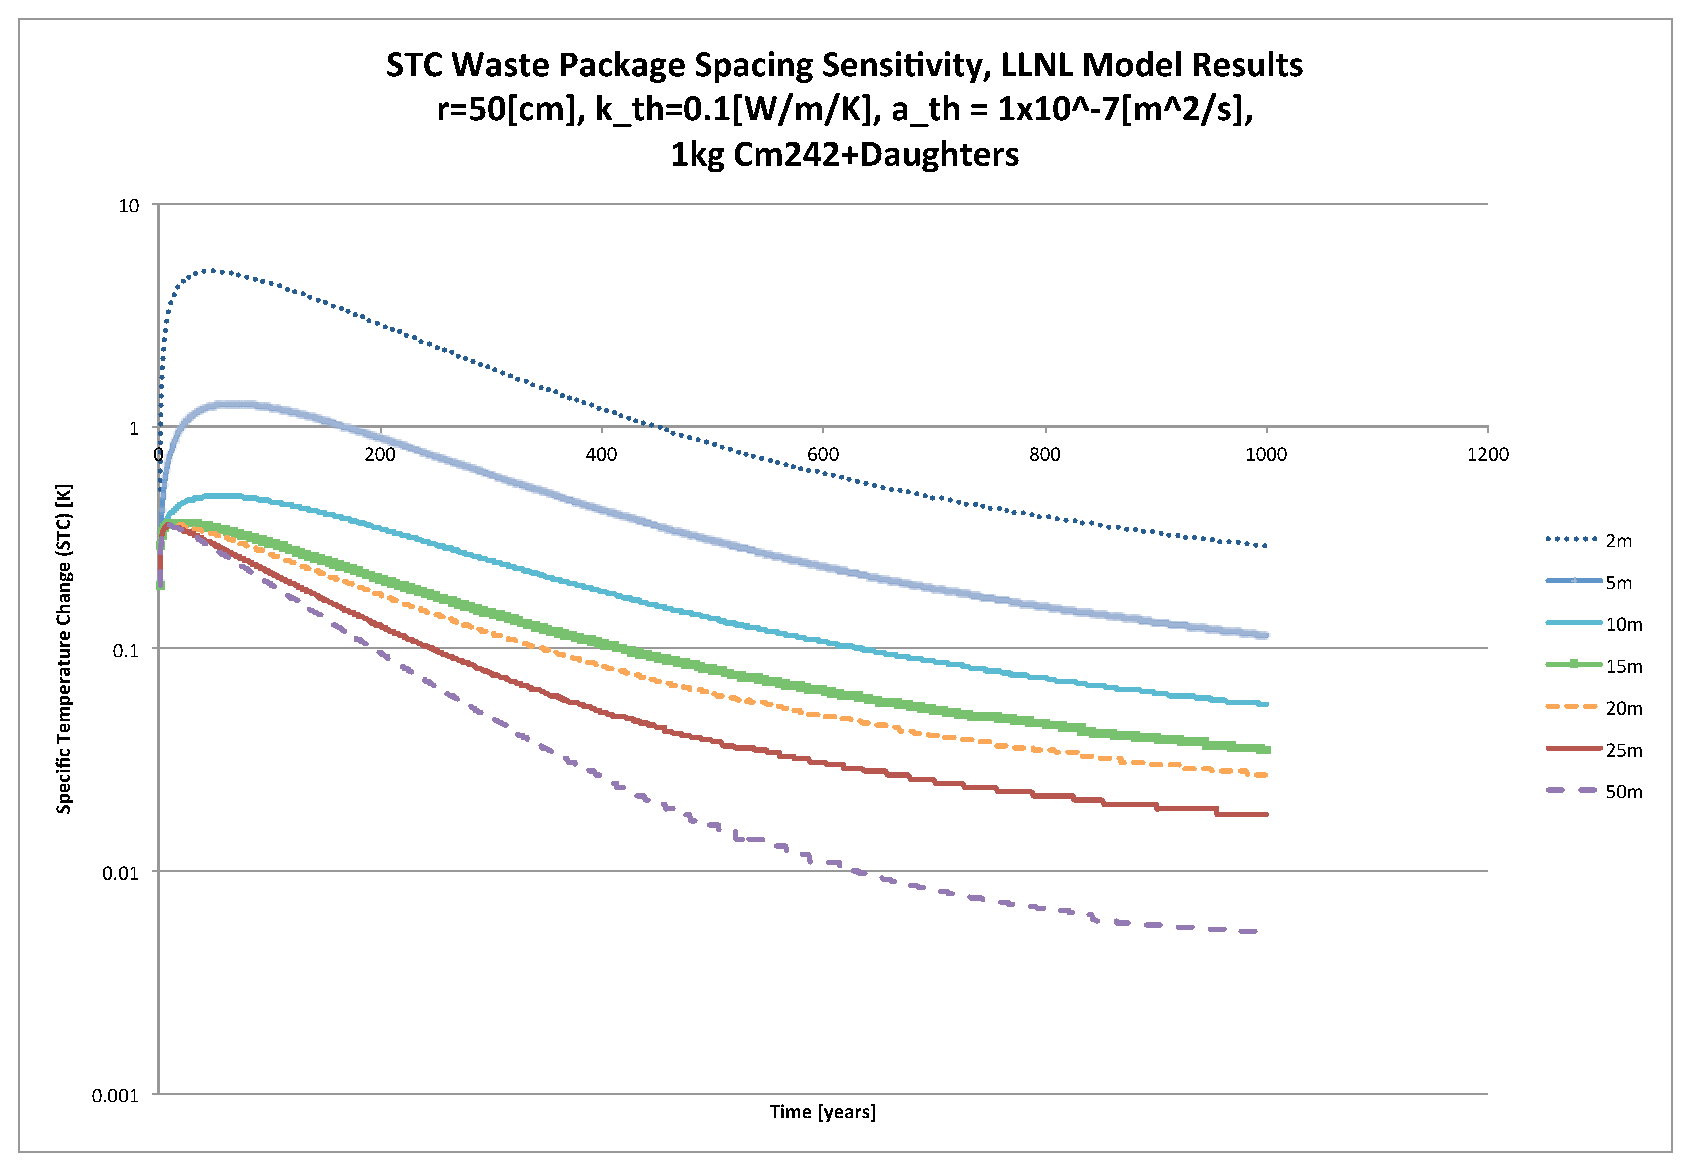
\includegraphics[width=0.7\textwidth]{./chapters/demonstration/spacing/Cm242spacing_sens.eps}
\end{center}
\caption[Thermal Sensitivity to $K_{th}$ and $s$]{Increased waste package 
spacing decreases temperature change 
(here represented by \gls{STC}) in the near field (here $r_{calc} = 0.5$ m).}
\label{fig:Cm242spacing_sens}
\end{figure}

Figure \ref{fig:Cm242spacing_sens} shows the trend in which increased waste 
package spacing of a medium decreases temperature change in the near field. This 
indicates that waste package spacing is an important parameter for repository 
concept design.  

Similarly, the location of the limiting radius has a strong effect on the 
waste package loading limit, for a fixed limiting temperature. In Figure 
\ref{fig:Cm242r_lim_sens}, the trend is demonstrated in which increased limiting 
radius (i.e. distance between the waste packages and the limiting radius) 
decreases the temperature at the limit, as expected.


\begin{figure}[htbp!]
\begin{center}
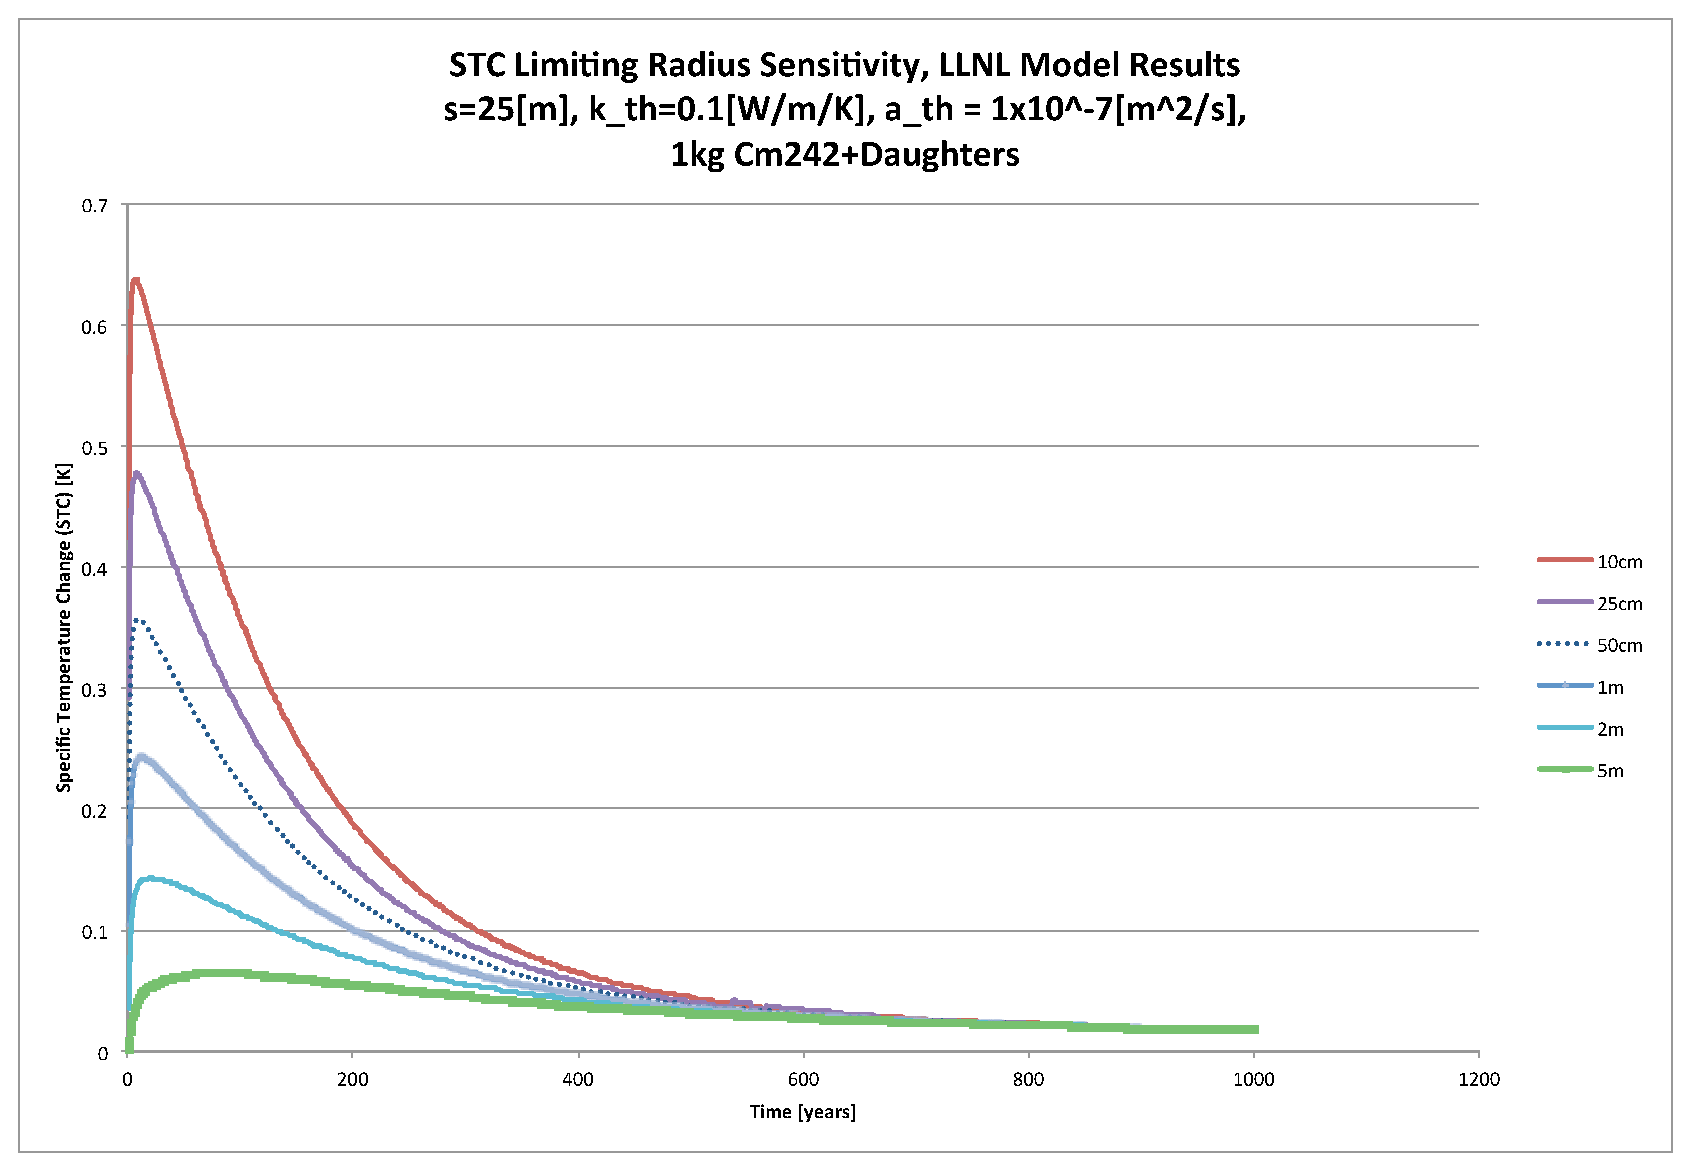
\includegraphics[width=0.7\textwidth]{./chapters/demonstration/spacing/Cm242r_lim_sens.eps}
\end{center}
\caption[Thermal Sensitivity to $r_{lim}$ and $s$]{Increased limiting radius 
decreases temperature change contributing to the thermal limit
(here represented by \gls{STC}).}
\label{fig:Cm242r_lim_sens}
\end{figure}


\FloatBarrier
\subsubsection{Cyder Results}


In a similar analysis, spacing and limiting radius were investigated. Figure 
\ref{fig:spacing_cyder} shows that the same spacing trend noted for the LLNL model was noted in the \Cyder model. 

\begin{figure}[htbp!]
\begin{center}
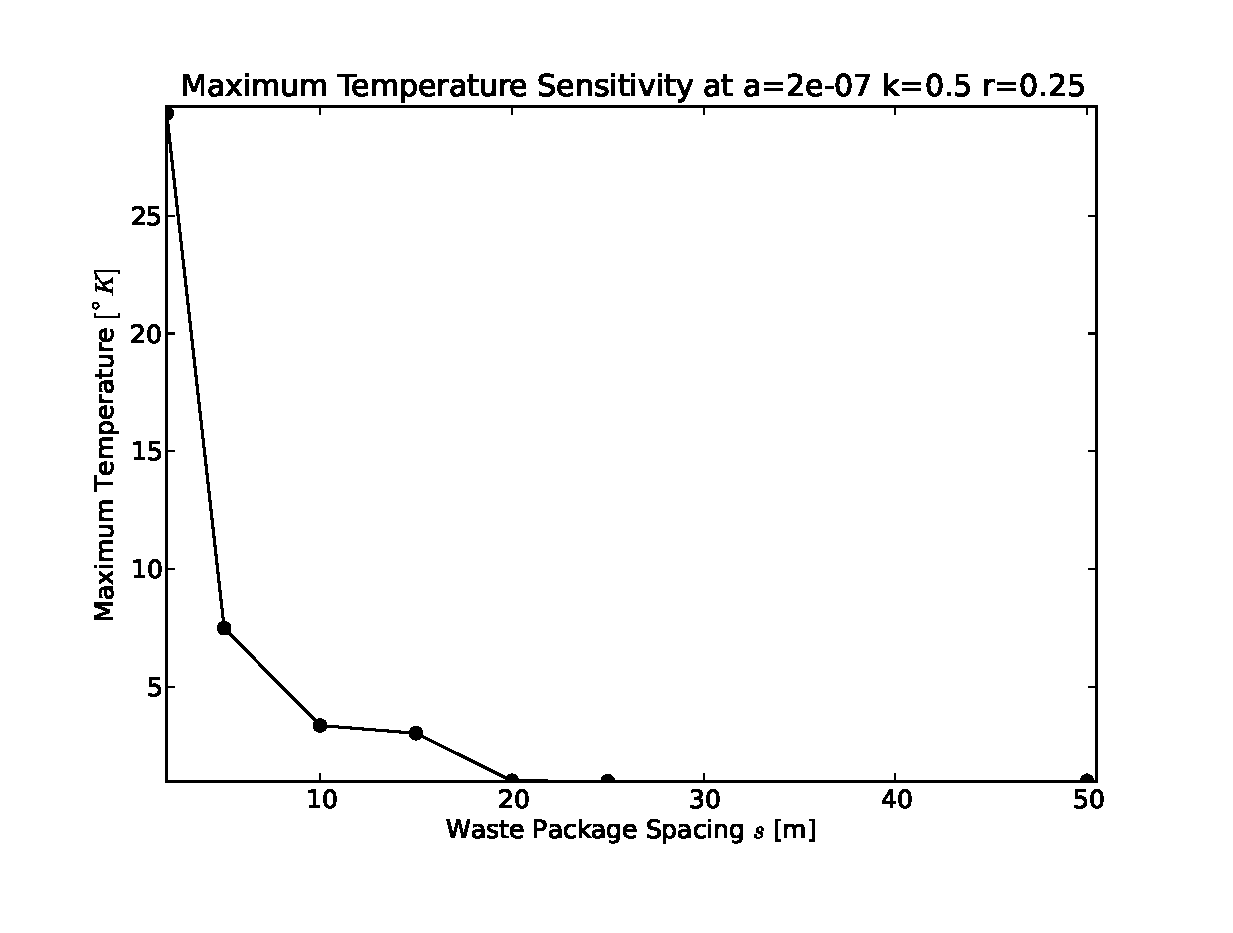
\includegraphics[height=0.7\textheight]{./thermal_demonstration/spacing/spacing.eps}
\end{center}
\caption[Spacing Sensitivity in Cyder]
{Cyder results agree with those of the LLNL model. The spacing between packages 
is inversely related to the temperature change in the medium at the limiting 
radius. The above example thermal profile results from 10kg of $^{242}Cm$.}
\label{fig:spacing_cyder}
\end{figure}


Similarly, figure \ref{fig:r_lim_cyder} shows the same trend for $r_{lim}$ in \Cyder as seen in the LLNL model.

\begin{figure}[htbp!]
\begin{center}
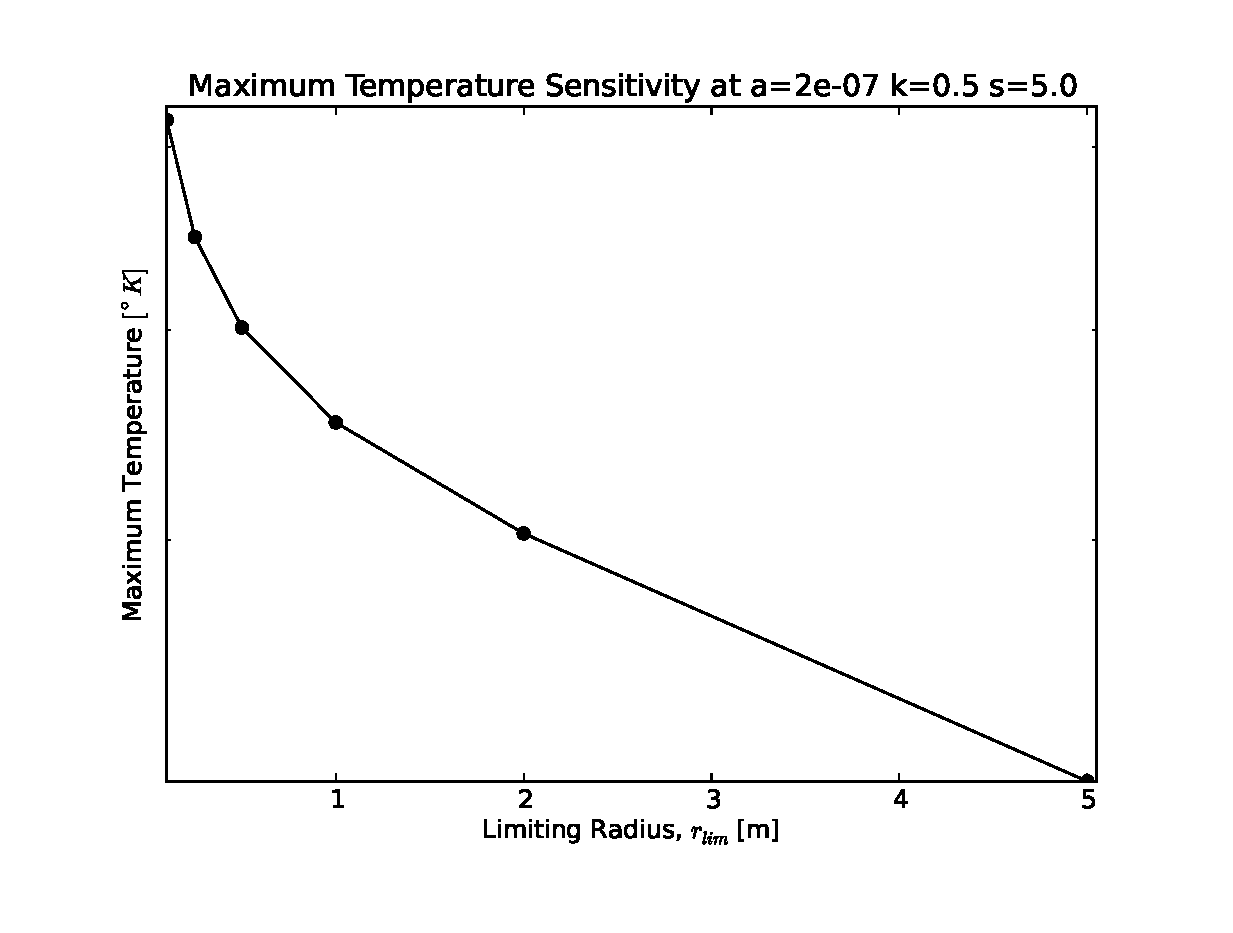
\includegraphics[height=0.7\textheight]{./thermal_demonstration/spacing/lim_radius.eps}
\end{center}
\caption[$r_{lim}$ Sensitivity in Cyder]
{Cyder results agree with those of the LLNL model. Increased limiting radius 
reduces the change in temperature at that radius. The above example thermal 
profile results from 10kg of $^{242}Cm$.}
\label{fig:r_lim_cyder}
\end{figure}
\end{frame}


In a similar analysis, the thermal diffusivity was compared both with the 
spacing between waste packages and the limiting radius. 

Figure \ref{fig:rs} validates the trend noted above that 
increased waste package spacing in a repository concept decreases areal thermal energy deposition 
in the near field.  Additionally, analysis with the \Cyder STC database 
demonstrates the way in which the importance of $r_{lim}$, the limiting radius, 
impacts the maximum calculated temperature at that radius. 

\begin{figure}[htbp!]
\begin{center}
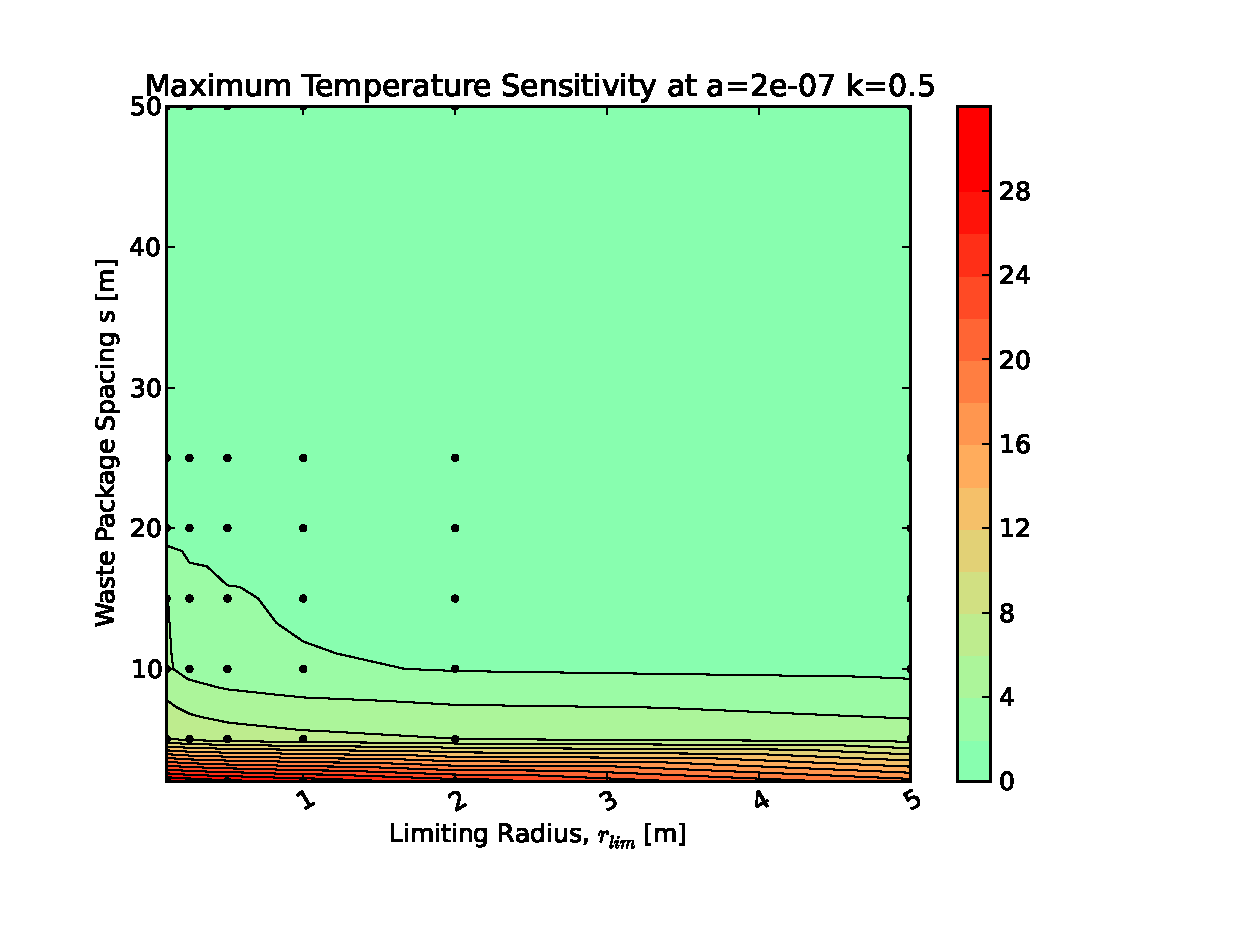
\includegraphics[width=0.7\textwidth]{./chapters/demonstration/spacing/rs.eps}
\end{center}
\caption[Thermal Sensitivity to $s$ and $r_{lim}$ Sensitivity in \Cyder]
{Cyder results agree with those of the LLNL model. The importance of the 
limiting radius decreases with increased $s$. The above example thermal 
profile results from 10kg of $^{242}Cm$}
\label{fig:rs}
\end{figure}
